% !TEX root = single_chapter_sn1006.tex
\chapter{SN1006}
\label{chap:sn1006}


\section{Introduction}

\citet{1980ApJ...241.1039S} identified an unusual O-Star (now called Schweizer-Middleditch Star, henceforth \smstar) near the centre of SN1006. After successful identifications of neutron stars in both the Vela Remnant and the Crab Remnant this was thought to be the third identification of a stellar remnant in ancient supernovae. Subsequent UV spectroscopy follow-up of the \smstar by \citet{1983ApJ...269L...5W} , showed strong \ion{Fe}{2}  with a profile broadened by a few thousand \kms. In addition, \citet{1983ApJ...269L...5W} identified redshifted \ion{Si}{2}, \ion{Si}{3} and \ion{Si}{4} lines. Their conclusion was that these absorption lines stem from an expanding iron core surrounded by a Silicon shell (similar what theoretical models suggest for a \sneia). This places the \smstar behind the remnant and it is thought to be unrelated to SN1006. 

\sn{1006} is the closest of the young \snia remnants. It's distance has been determined to 2.2\,\kpc\ by using optical proper motion methods and radial velocity measurements from the remnant expansion \cite{2003ApJ...585..324W}. The remnant of \sn{1006}{} has been very well studied in many aspects. Absorption lines of the remnant plasma can be seen in background UV sources. This has enabled \citet{2005ApJ...624..189W} to sketch the inner structure of the ejecta. A few tenth of a solar mass of iron suggests that this event was a \snia. The lack of a compact stellar remnant, similar to those found in \snii remnants, also suggests a thermonuclear event. 

\sn{1006}{} provides the perfect site for a donor star search. High extinction values that introduce additional challenges to stellar analysis (as seen in the \sn{1572}{} remnant) are not present. The extinction, estimated for the background \smstar, is relatively low  at E(B-V) = 0.1 \citep{1993ApJ...416..247W,2003ApJ...585..324W}. These serendipitous conditions for the \sn{1006}{} remnant led us to launch a photometric and spectroscopic campaign to search for the donor star. The photometric observations were taken at Siding Spring Observatory with the 2.3m Telescope imager. The spectroscopic search area was determined by the center of the \snr{1006}{} and a radius (see Figure \ref{fig:overview_sn1006}). For the center we have opted to adapt a center determined by the mean of the \xray\ and radio center presented in \citet{2003ApJ...585..324W}. As a radius we have opted to use 75\arcsec, which translates into 2000\,\kms at the distance of \sn{1006}{}. We do believe that this generously chosen radius takes uncertainties of the center as well as the donor star scenarios into account. The spectroscopic observations were undertaken with the FLAMES multi-object spectrograph.

\begin{figure}[htbp] %  figure placement: here, top, bottom, or page
   \centering
   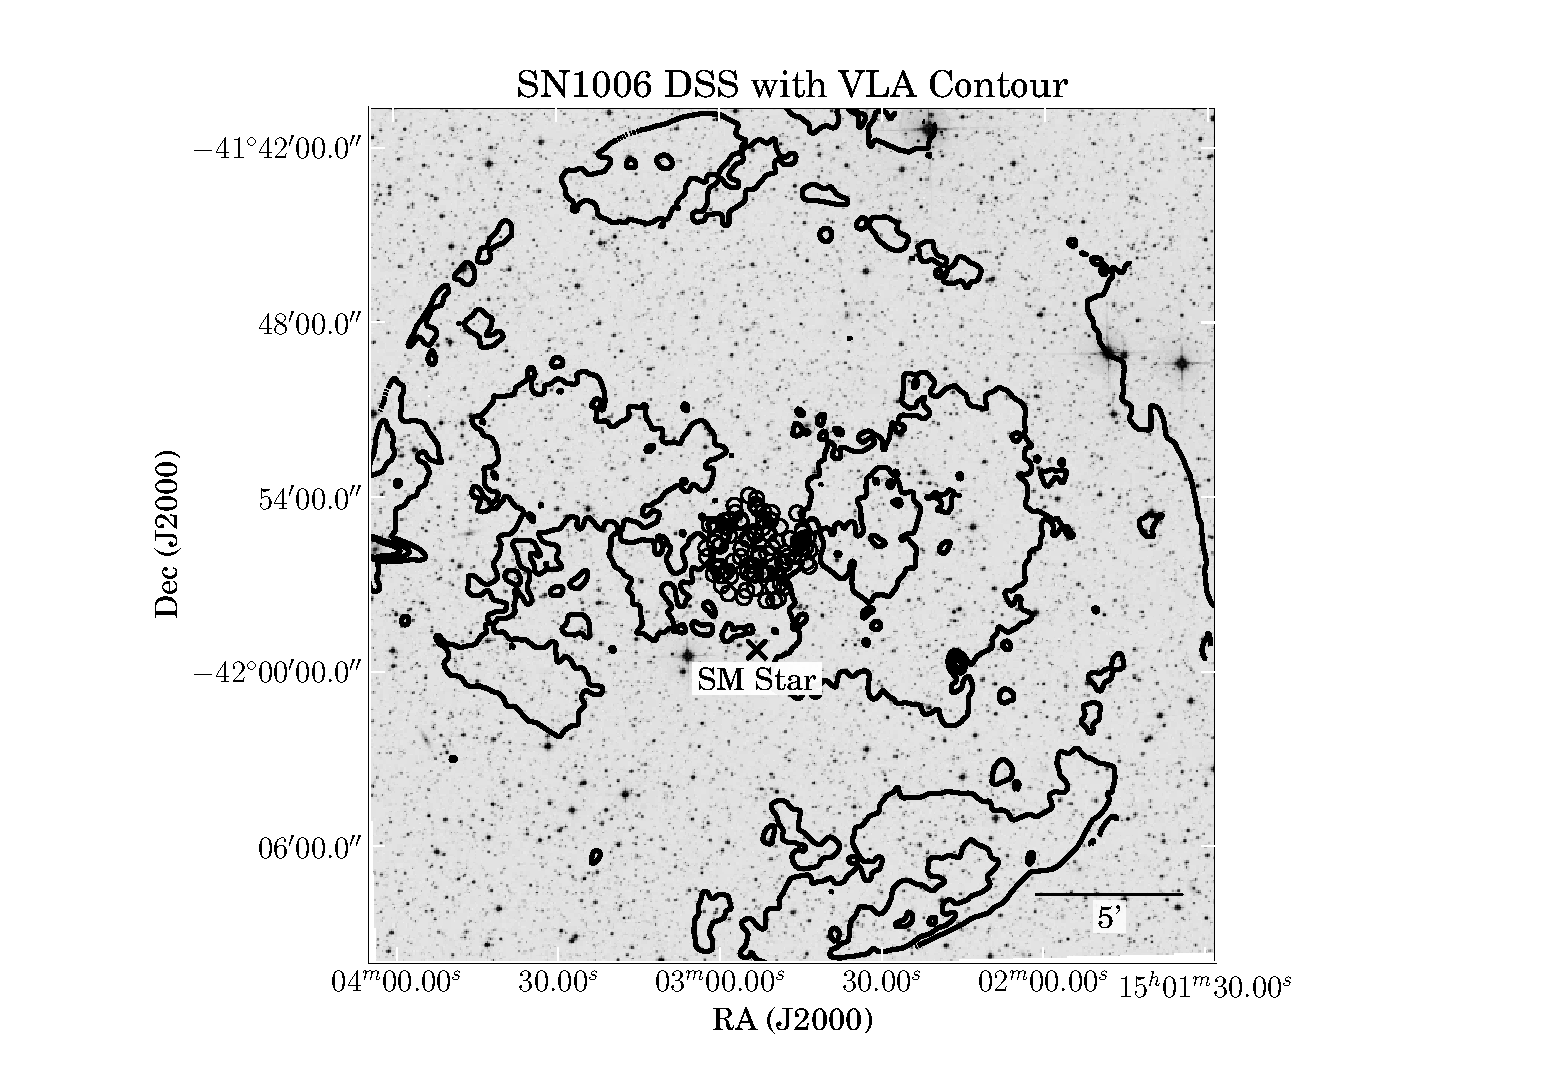
\includegraphics[width=0.8\textwidth]{chapter_sn1006/plots/sn1006_overlay_withsm.pdf} 
   \caption{example caption}
   \label{fig:overview_sn1006}
\end{figure}

We present photometry as well as high-resolution spectroscopy of the stars in SN1006 (for an overview see Figure \ref{fig:overview}. In Section \ref{sec:obs_and_red} we outline the observations as well as data reduction of the photometric and spectroscopic data. Section \ref{sec:analysis} is split into five subsections. We first describe the photometric analysis and radial velocity measurements. The complete analysis of the data has not been done and we mainly present our analysis technique. We do, however have some initial results which we will outline in Section blah. We conclude this chapter in Section \ref{sec:conclusion} and discuss the possible implications of our initial find. In addition, we will describe future work including the final analysis of the data 


\section{Observations and Data Reduction}

For our spectroscopic survey we selected 79 stars in a 75 \arcsec radius (this corresponds to 780\,\kms at a distance of 2.2\,\kpc) around the centre of SN1006 ($\alpha = \rasc{15}{02}{22}{1};\delta = \decl{-42}{05}{49}$). We observed targets to a maximum magnitude of R=18, this translates to a limiting luminosity of $L=L_{\textrm{R}_\odot}$. The surviving donor scenarios described in \citet{2000ApJS..128..615M} and \citet{2008A&A...489..943P} should be easily visible. 
The VLT instrument FLAMES provides high resolution (R=25,000) and a large field of view (25\arcmin) for a considerable number of stars per setup (130 targets). We chose the wavelength region from 5139\,\AA\ to 5356\,\AA\ which contains the gravity sensitive MgB Triplet as well as many Fe-Lines to accurately measure metallicity. Fibre buttons can be placed no less than 11\arcsec\ apart. Thus to observe all of the program stars in the crowded central field, we split the stars over three different setups. The first two setups were observed five times with 2775 s each. We deliberately chose bright stars for the last setup so that it only had to be observed three times with 2775 s each. As only the central 75\arcsec were crowded we placed spare fibres on three bright stars (R$\approx 10$; 2mass J15032744-4204463, J15031746-4204165, J15033195-4202356) located close to the edge of the 25\arcmin field for calibration purposes. Additional spare fibres were placed on sky positions. These were determined to be far from \twomass\ sources and were subsequently manually inspected using DSS images (citedss). 

We requested standard daytime calibration as well as simultaneous arc exposures with four fibres for each observation block. There are 13 observation blocks with an exposure time of 2775 s each. Table \ref{tab:observations} provides the Observing ID, modified julian date, mean seeing, mean airmass, setup name and heliocentric correction for all observations. 
Due to broken fibres not all stars where observed for the expected length of time. \candstar{31} was not observed at all in this sample (see Figure \ref{fig:zoomed_overview_sn1006} for the observation of the center of SN1006. This).

We applied a cosmic ray removal tool on the raw 2D frames \citep{2001PASP..113.1420V}. 
The data was then reduced with the ESO-CPL pipeline (version 5.2.0), using the GIRAFFE instrument recipes (version 2.8.9). The only change that was made to the default parameters was the usage of the Horne extraction algorithm instead of the "Optimal"-extraction algorithm. This yielded 366 individual spectra of the candidate stars and an additional 39 spectra of the Calibration stars. 
In addition,  the Giraffe pipeline yields error frames which were used in the fitting process described in Section \ref{sec:sn1006_stelparam}. 
\begin{deluxetable}{cccccc}
\tablecaption{Observations}
\tablehead{\colhead{ObsID} & \colhead{MJD} & \colhead{FWHM} & \colhead{Airmass} & \colhead{SetupName} & \colhead{$\Delta v_{\rm helio}$}\\ 
\colhead{-} & \colhead{d} & \colhead{\arcsec} & \colhead{-} & \colhead{-} & \colhead{\kms}}


\startdata
360737 & 54965.1 & 1.2 & 1.2 & SN1006 1 & 1.5\\
360739 & 54965.1 & 1.2 & 1.1 & SN1006 1 & 1.5\\
360740 & 54965.1 & 1.0 & 1.1 & SN1006 1 & 1.4\\
360741 & 54985.0 & 0.7 & 1.4 & SN1006 1 & -7.4\\
360742 & 54964.2 & 1.5 & 1.1 & SN1006 1 & 1.7\\
360743 & 54985.0 & 0.8 & 1.2 & SN1006 2 & -7.5\\
360745 & 54985.0 & 0.9 & 1.1 & SN1006 2 & -7.6\\
360746 & 54985.1 & 1.0 & 1.1 & SN1006 2 & -7.7\\
360747 & 54985.1 & 1.0 & 1.1 & SN1006 2 & -7.7\\
360748 & 54985.2 & 0.9 & 1.1 & SN1006 2 & -7.8\\
360749 & 54963.1 & 1.2 & 1.2 & SN1006 3 & 2.4\\
360751 & 54963.1 & 1.1 & 1.1 & SN1006 3 & 2.3\\
360752 & 54963.2 & 1.1 & 1.1 & SN1006 3 & 2.3\\
\enddata
\label{tab:observations}
\end{deluxetable}


Our photometry was deduced from images taken with the image at the 2.3m Telescope at the Siding Spring Observatory. All data was taken on the night of the 11th of May. We exposed for 1860 s in U-Band, 1490 s in B-Band, 788s in V-Band and 1860 s in I-Band. For calibration purposes we took images of the PG1633 and PG1047 standard star regions in the same filters. The seeing ranged between 1 and 2 \arcsec. 

The data was reduced in the standard way using PyRAF \footnote{PyRAF is a product of the Space Telescope Science Institute, which is operated by AURA for NASA.}.

Finally an astrometric solution was fitted using astrometry from the \twomass\ point source catalogue \citep{2006AJ....131.1163S}. 


\section{Analysis}

A uniform analysis of this set of data is technically challenging due to the large variation in spectral quality (see Figure \ref{fig:sn1006_comparespec}). We have explored multiple channels and believe that, although challenging, it is possible. We measure the radial velocity using the standard technique of cross-correlation \citep{1979AJ.....84.1511T}. 
It is crucial in our set to measure rotation, as this is one of key features of potential donor stars. In addition, a giant star with high rotation can be incorrectly identified as a main-sequence star without rotation. We are currently trialling multiple techniques for measuring stellar rotation. For identifying the fundamental stellar parameters we use a standard grid based approach. 

\subsection{Photometry}
We used SExtractor \citep{1996A&AS..117..393B} to measure the magnitudes of the objects in the frames. We used the Stetson magnitudes \footnote{This research used the facilities of the Canadian Astronomy Data Centre operated by the National Research Council of Canada with the support of the Canadian Space Agency}  of our standard fields PG1633 and PG1047 to calibrate our magnitudes to a standard Bessel Filter system. 

The measured  magnitudes were supplemented with near infrared magnitudes from the \twomass\ point source catalogue.
To check the photometric measurements we plotted the obtained B-V colours against the V-K colours and compared this to theoretical colours from \citep{2010A&A...512A..54C} in Figure \ref{fig:colour_check}.  \candstar1006{60} presents a strong outlier in this case. Inspecting our as well as 2MASS imagery we believe there to be a second source which would explain this behaviour. 

To compute temperatures from photometric colours we used the polynomials given in  \citep{2010A&A...512A..54C} and assumed an \feh=0 for all stars in the first instance. The temperature polynomial coefficients incorporating the metallicity are particularly small for the V-J colour. If V-K was not available (as 2MASS did only provide upper limits for some of our program stars) we tried to use V-J colours. 

The photometry and temperature estimates can be seen in Table \ref{tab:photometry}
\subsection{Proper motion}
Do we have proper motions. We claimed to have some to an accuracy of 10 mas/yr

\subsection{Radial Velocity}

To obtain radial velocities we employ a two step process. We first used a solar spectrum from Hinkel et al with sn ... r .... . 
We used the standard cross-correlation technique described in \citep{1979AJ.....84.1511T} and implemented in the IRAF-task \textit{fxcor}. The cross-correlation was performed on every single spectra. The results were then averaged for each star, employing a sigma clipping algorithm. 

We note that especially for faint objects we observe a second cross-correlation peak at 0\,\kms and believe that this is reflected light from the moon which was visible for all our observations. 

In a second step we will use the matching stellar parameters and construct a matching synthetic template to improve the accuracy of our measurement. We do not believe this to change by much. 

In Figure \ref{fig:vrad_comp} we have compared our radial velocity measurements with the Besan\c{c}on kinematic model of the Milky way \citep{2003A&A...409..523R}. Our selection criteria was all stars within a circle with an area ???square degree?? around the center of SN1006 and a magnitude cut of V$>$10. We compared the resulting 16400 stars to our 78 stars in the sample. 
 
None of the stars show any particularly peculiar radial velocity. We note however that the spread in radial velocity in this direction is large and that a potential donor star might not be visible as a kinematic outlier. 

\subsection{Rotational Velocity}
A distinguishing feature for a donor star is thought to be rotation Kerzendorf 2009. As pointed out in section \ref{sec:radvel} radial velocity especially in the direction of SN1006 might not be an identifying attribute as it has a large distribution. 

!!! first describe psd method then go to better method .... .
We can describe the rotation in a stellar spectrum with a convolution of a non-rotating star with a rotational profile. This rotational profile will broaden with wavelength. For our relatively small spectral region, however, we assume it to be constant. 
A convolution can be described in Fourier space in the following way,
\[
	F(f \otimes g) = F(f) \times F(g), 
\]
where $F$ denotes the fourier transform and f and g are functions. When comparing a synthetic spectrum in fourier space to one of the observed spectra it is possible to measure the convolution function. The lower the S/N-ratio however the harder it becomes to measure the rotation (see Figure \ref{fig:psd_vs_sn}). To lower the noise in the fourier transformed spectrum we employed Welch's method \cite{1967ITAE...15...70W}. This method splits the spectrum into overlapping sections, which are then mutliplied with a window function (in our case the Hann function) and finally fourier transformed. These transformed segments are then averaged. This reduces removes the low frequencies and reduces frequency resolution. In our case, however, we are interested in high frequency caused by the line profiles. 

In addition to rotational broadening the instrument introduces a broadening which is described by the resolution of the instrument. Thus before measuring rotational velocity we broadened our synthetic spectra with the nominal resolution and checked the result in Fourier space. 

Finally, the rotation was measured by comparing a synthetic spectrum broadened with a rotational kernel to the measured spectrum until they agreed. 

This method was successful in attaining the rotational velocity in low S/N synthetic spectra, but has not yet been applied successfully to the observed spectra.

The rotation measured by John laird ??? using a different method is displayed in ......


\subsection{Stellar Parameters}
\label{sec:sn1006_stelparam}
As an initial approach we used: 

Describe LAIRD method

----------
To get more detailed stellar parameters we employed a technique using a grid in \teff, \logg\ and \feh. 
\moog \citep{1973ApJ...184..839S} was used to synthesize the spectral grid using the model stellar atmospheres by \citet{2003IAUS..210P.A20C}. Line wings were taken into account up to 8\,\AA away from line centre, which seemed to be a reasonable compromise between grid creation and accuracy. For the atomic lines we merged values from the VALD-2 database \citep{2000BaltA...9..590K} with adjusted values (to reproduce the Arcuturs and the Sun) from \cite{2008A&A...486..951G}. We used the measured
molecular lines described in  \citet{1995KurCD..23.....K}. 
The grid extends from 3500\,K to 7500\,K in \teff with a stepsize of 250\,K, in \logg\ it ranges from  0 to 5 with a stepsize of 0.5 and in \feh\ it ranges from -2.5 to 0.5 with a stepsize of 0.5 (with an extra set of points at 0.2). 

We used the appropriate sections from the solar spectrum \citep{1984sfat.book.....K} and the arcturus spectrum  \cite{2000vnia.book.....H} to calibrate our spectral grid. 
Before fitting against the grid we broadened both sun and arcturus spectra and the synthetic spectra to the resolution of our observed spectra. 

We determined stellar parameters by first finding the best fitting grid point and then using the minimizer MINUIT to find a minimum by interpolating between the gridpoints \citep[using][]{Barber96thequickhull}. For a more detailed explanation of the n-dimensional interpolation see chapter \ref{chap:qhull}. For the Sun we obtain stellar parameters of \teff=5825\,K, \logg=4.4 and \feh=-0.12 and for Arcturus we obtain stellar parameters of \teff=4336\,K, \logg=1.9, \feh=-0.67. 
We acknowledge the error in measurement, but believe our spectral grid to be accurate enough for distinguishing a potential donor candidate. 

To measure our observed spectra we need to first fit the continuum. We decided for a Legendre polynomial with a maximum order of 3 and a sigma clipping algorithm. The order that gave the lowest RMS of the fit was used. After determining initial parameters we would divide by synthetic spectrum with these parameters and fit the continuum again as some parameters (like \feh) are very continuum sensitive.  

For now we have only measured stellar parameters for synthetically created spectra using the real sun and arcturus spectra as an input. We multiplied these spectra with an artificial continuum and introduced artificial noise to recreate a S/N-ratio of 5 (similar to the measure low S/N spectra). The results can be seen in Figure \ref{fig:sparam_sun_arcturus}.


\subsection{Distance Measurements}

Similar to Kerzendorf et al 2011 we plan to use synthetic magnitudes derived from isochrones to give an estimate of distance. 
We 

\section{Conclusions}

The initial measurements do not show any obvious donors. 

